\documentclass[10pt,twocolumn]{article}
\usepackage[T1]{fontenc}
\usepackage[utf8]{inputenc}
\usepackage{amsmath,amssymb,booktabs,graphicx,url,microtype,enumitem}
\usepackage[margin=0.62in,columnsep=0.22in]{geometry}
\setlength{\parindent}{1em}
\setlength{\parskip}{0pt}
\setlist{nosep,leftmargin=*}
\title{\vspace{-1.3em}\textbf{When Process Gains Fail to Improve Coding Agents:\\A Replicated Intervention Study}}
\author{Prakash Verma}
\date{}
\begin{document}
\maketitle
\vspace{-1.5em}

\begin{abstract}
Coding-agent interventions are often judged only by final task success, obscuring whether a treatment was executed and whether it changed the intended process. We study a frozen Gemma 4 31B software-engineering agent using controlled interventions for edit recovery, workspace-correct verification, graph localization, patch restraint, and semantic falsification. The main corpus contains 416 trajectories across 91 issues; 356 controlled/stress trajectories cover 43 issues. Edit recovery raises non-empty patches from 42/60 to 49/60 but resolution only from 16/60 to 17/60; 8/10 rescued empty-patch cases remain unresolved, and an initial 10/30 versus 8/30 advantage reverses to 7/30 versus 8/30. On the shared 30-task cohort, 5 issues resolve in all 11 batches, 20 in none, and 5 vary; baseline and intervention solved-task unions are the same 10 issues. Naive trace matching also overstates semantic-falsification uptake from 5/30 executed checks to 30/30. We therefore separate assignment, uptake, mechanism shift, correctness, and replication when evaluating agent interventions.
\end{abstract}

\section{Introduction}
A benchmark score alone does not reveal whether an intervention changed localization, editing, verification, or only the prompt. We ask: \emph{when an intervention measurably changes an intermediate agent process, does that change propagate to correct repairs?} Using one frozen Gemma 4 31B agent, we separate \textbf{assignment}, \textbf{uptake}, \textbf{mechanism shift}, \textbf{correctness}, and \textbf{replication}.

Four findings recur: rescued edits often remain incorrect; small gains reverse under replication; interventions do not expand the observed solved-task set on the shared cohort; and prompt assignment can differ sharply from executed uptake.

\begin{figure*}[t]
\centering
\small
\setlength{\tabcolsep}{5pt}
\begin{tabular}{ccccc}
\fbox{\parbox[c][0.62in][c]{0.17\textwidth}{\centering\textbf{Assignment}\\4 operational + 1 semantic prompt}} &
$\rightarrow$ &
\fbox{\parbox[c][0.62in][c]{0.20\textwidth}{\centering\textbf{Executed uptake}\\Verify 13/13; graph 12/30; falsification 5/30}} &
$\rightarrow$ &
\fbox{\parbox[c][0.62in][c]{0.18\textwidth}{\centering\textbf{Mechanism shift}\\Non-empty patches 70.0\% $\rightarrow$ 81.7\%}} \\
\\[-1pt]
&& $\downarrow$ && \\
\\[-1pt]
\multicolumn{2}{c}{} &
\fbox{\parbox[c][0.62in][c]{0.20\textwidth}{\centering\textbf{End-task correctness}\\Resolution 26.7\% $\rightarrow$ 28.3\%; 2/10 rescues}} &
$\rightarrow$ &
\fbox{\parbox[c][0.62in][c]{0.18\textwidth}{\centering\textbf{Replication}\\10/30 vs 8/30 $\rightarrow$ 7/30 vs 8/30}}
\end{tabular}
\caption{Five-stage evaluation framework with representative observed process and outcome changes.}
\label{fig:framework}
\end{figure*}

\section{Experimental Setup}
\textbf{Agent.} All controlled runs use the same single Gemma 4 31B agent (\texttt{gemma-4-31b-it-qat-w4a16-ct}), temperature 0.2, thinking budget 4096, 28 counted tool calls, 80 turns, and an 8-minute limit. The tool interface includes file read/edit/write, shell execution, status/submission, and three code-graph/search tools.

\textbf{Corpus.} The complete frozen analysis contains 416 trajectories across 91 unique issues in FastAPI, Rich, Requests, and HTTPX. Sixty exploratory trajectories motivate hypotheses. The controlled/stress subset contains 356 trajectories across 43 unique issues in FastAPI, Rich, and Requests: 120 initial four-condition runs, 60 edit-recovery replication runs, 26 targeted Requests verification runs, 60 forced-localization runs, 60 semantic-restraint runs, and 30 semantic-falsification runs. The initial four-condition study also included preliminary verification-path and graph-prompt arms, each resolving 7/30 versus an 8/30 baseline. Because the former cohort contained no Requests/HTTPX import-shadowing cases and the latter produced no graph-tool uptake, the later targeted studies replace them for mechanism-specific interpretation.

\textbf{Interventions.} Edit recovery instructs the agent to recover from failed edits with a re-read and smaller retry. Workspace verification uses \texttt{PYTHONPATH=src} and \texttt{\_\_file\_\_} checks when import shadowing is possible. Forced localization requests graph use before editing. Semantic restraint asks for minimal scope and preserved behavior. Semantic falsification asks for an adversarial counterexample check before final submission.

\textbf{Fresh-task semantic diagnostic.} A separate diagnostic uses 12 previously unused evaluation issues (10 FastAPI, 2 Rich), each run twice under two conditions. Operational control (O) retains edit recovery, workspace-import verification, and generic behavioral-review guidance; that guidance also asks the agent to prefix its focused check with \texttt{CONTROL\_BEHAVIOR\_CHECK}. O+S is identical but adds a frozen, self-reviewed behavioral checklist and requests \texttt{SPECIFICATION\_DRIVEN\_CHECK}; the checklist was derived only from the issue statement before inference, with no reference patch, hidden test, evaluator output, or candidate-run outcome. Two pre-specified preflight issues (one FastAPI, one Rich; four total O/O+S runs) were used only to debug the harness and were excluded before evaluation began.

\textbf{Statistics.} Resolution comparisons are paired by task. We report exact discordant-pair tests for each controlled study. Pooled repeated-task summaries are descriptive because the same 30 issue IDs are reused across repetitions. Conditional quantities such as $P(\mathrm{resolved}\mid\mathrm{patch})$ are descriptive because patch production is post-treatment. With only 30 paired issues in the main comparisons and few discordant outcomes, the study has limited sensitivity to modest improvements; for a two-sided exact discordant-pair test, even five discordant pairs all favoring one condition give $p=0.0625$, while six give $p=0.03125$. Failure to detect a reliable gain should therefore not be read as evidence of equivalence.

\section{Results}
\subsection{Process changes do not reliably propagate to resolution}
Table~\ref{tab:main} places each targeted process shift beside its paired outcome. Several interventions clearly change the intended process, but no reliable improvement in resolution is detected at these sample sizes.

\begin{table*}[t]
\centering
\small
\caption{Controlled interventions. Process metrics and paired resolution outcomes are reported separately.}
\label{tab:main}
\begin{tabular}{lllllll}
\toprule
Experiment & Process shift & Base & Int. & Base-only & Int.-only & Exact $p$ \\
\midrule
Edit recovery (initial) & empty patches $10/30\to5/30$ & 8/30 & 10/30 & 0 & 2 & 0.50 \\
Edit recovery (repl.) & empty patches $8/30\to6/30$ & 8/30 & 7/30 & 1 & 0 & 1.00 \\
Requests verification & \texttt{PYTHONPATH=src} $2/13\to13/13$ & 1/13 & 1/13 & 0 & 0 & 1.00 \\
Forced localization & pre-edit graph $0/30\to12/30$ & 6/30 & 7/30 & 1 & 2 & 1.00 \\
Semantic restraint & empty $7\to10$; med. chars $611\to549$ & 8/30 & 8/30 & 1 & 1 & 1.00 \\
\bottomrule
\end{tabular}
\end{table*}

\subsection{Edit recovery moves failures downstream}
Pooling the two edit-recovery experiments, baseline produces non-empty patches in 42/60 runs (70.0\%) and resolves 16/60 (26.7\%). Edit recovery produces non-empty patches in 49/60 (81.7\%) and resolves 17/60 (28.3\%). Descriptively,
\[
\begin{aligned}
P(\mathrm{resolved}\mid\mathrm{patch})_{\mathrm{base}} &= 16/42 = 38.1\%,\\
P(\mathrm{resolved}\mid\mathrm{patch})_{\mathrm{recovery}} &= 17/49 = 34.7\%.
\end{aligned}
\]
Because patch production is post-treatment, this conditional comparison is not causal. The cleaner paired audit is the transition set itself: 10 task-runs move from baseline-empty to intervention-nonempty, but only 2/10 resolve. Three transitions occur in the opposite direction; all three baseline patches were already unresolved.

Pooling the two repetitions gives 17/60 resolved under edit recovery versus 16/60 under baseline, a descriptive difference of $+1.7$ percentage points. Because these 60 runs reuse the same 30 issues, we do not treat them as 60 independent observations. Patch production increased in both repetitions, while resolution changes were small and changed direction.

\begin{figure}[t]
\centering
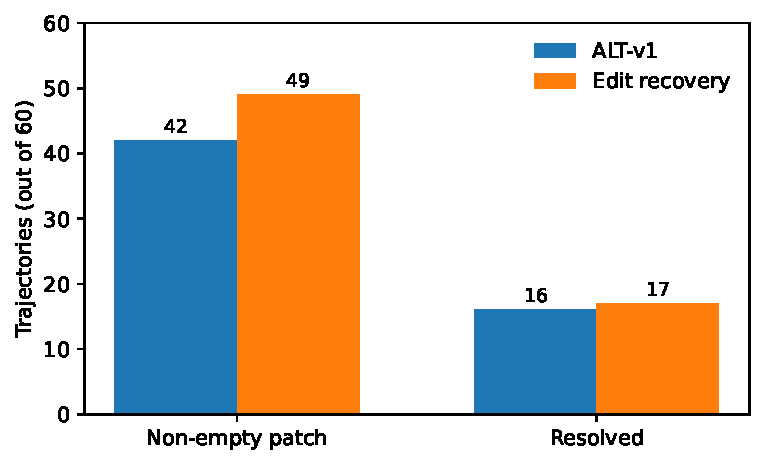
\includegraphics[width=0.96\columnwidth]{edit_recovery_funnel_camera_ready.pdf}
\caption{Edit recovery increases patch production much more than final resolution.}
\label{fig:funnel}
\end{figure}

\subsection{Replication changes the interpretation}
The initial edit-recovery run favors the intervention 10/30 versus 8/30. Repeating the same frozen 30-task cohort yields 7/30 versus 8/30. Across the four baseline/intervention cells from these two repetitions, only three issues---\texttt{rich\_3063}, \texttt{rich\_3180}, and \texttt{rich\_3278}---change resolved status; the other 27 are stable. Thus the apparent aggregate gain and reversal are concentrated in a very small set of tasks. Aggregate stability can therefore hide task-level stochasticity.

Semantic restraint shows the same caution from another angle: both conditions resolve 8/30, with one task favoring each side. With only two discordant tasks, the exact paired test is uninformative about modest effects; this result supports uncertainty, not equivalence.

\subsection{Post-hoc sensitivity: solved frontier and patch-size composition}
Two descriptive post-hoc analyses test whether apparent process gains reflect broader capability or changes in which runs produce outputs. On the shared 30-task cohort, four independent ALT-v1 repetitions yield 30 successful runs across 120 attempts and solve 10 distinct issues at least once. Seven intervention batches yield 53 successful runs across 210 attempts but also solve only 10 distinct issues. Across the 11 batches, resolved counts range from 6 to 10 (mean 7.55, sample SD 1.04), so a one- or two-task difference between individual 30-task batches is comparable to the observed batch-to-batch variation. The 20 issues never solved by any baseline repetition produce zero resolutions across 140 intervention attempts, giving 0/220 across baseline-plus-intervention attempts on those same issues. Their failures are heterogeneous: 67/220 attempts produce an empty patch, 46/220 encounter an agent timeout/tool/turn limit, and 197/220 record evaluator exit code 1 or 2; these categories overlap. Across all 11 shared-cohort batches, 5 issues resolve every time, 20 never resolve, and 5 vary. Thus, interventions change individual run outcomes without expanding the \emph{observed} solved-task set on this frozen cohort. This is descriptive and post-hoc; it does not imply that the remaining 20 issues are intrinsically unsolvable.

\begin{figure*}[t]
\centering
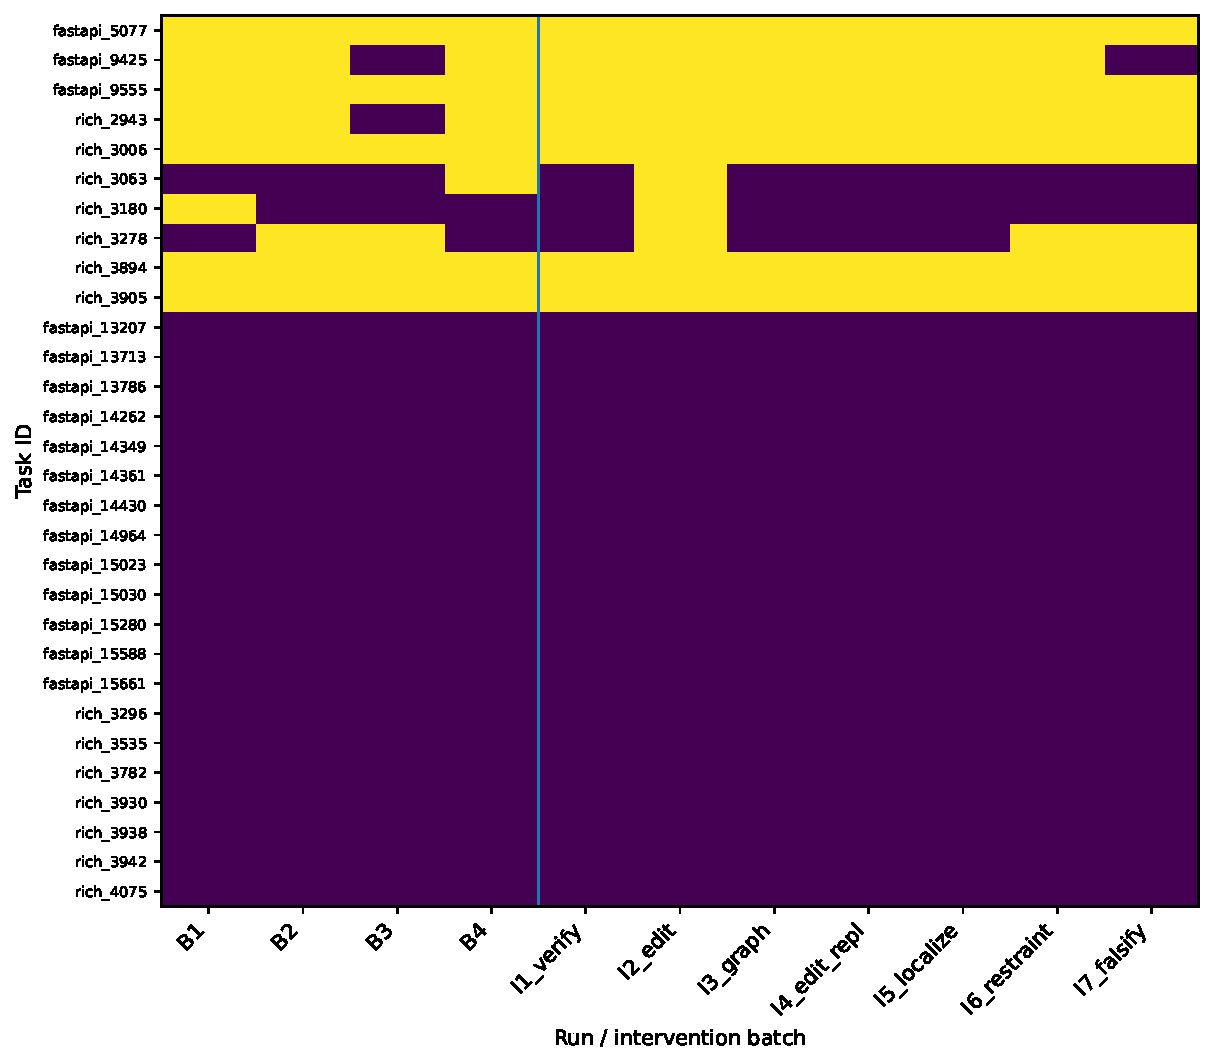
\includegraphics[width=0.82\textwidth]{solved_frontier_heatmap.pdf}
\caption{Task-level resolution matrix for four baseline repetitions (B1--B4) and seven intervention batches (I1--I7) on the shared 30-task cohort. The same 10 issues are solved at least once by baseline and by interventions; the 20 baseline-never-solved issues remain unsolved across 140 intervention attempts. This analysis is descriptive and post-hoc.}
\label{fig:frontier}
\end{figure*}

Patch-size restraint shows a related compositional effect. The unconditional median patch size falls from 611 to 549 characters, but empty patches increase from 7/30 to 10/30. Restricting descriptively to non-empty outputs, medians are 895 and 891.5 characters. Among the 18 tasks with non-empty patches in both conditions, the median paired change is zero: 8 patches shrink, 4 are unchanged, and 6 grow. The lower unconditional median therefore largely reflects a change in which runs produce patches rather than a consistent reduction in comparable patch size.

Together, these analyses show that aggregate process gains can coexist with ordinary batch variation, a fixed solved-task frontier, and little like-for-like output improvement.

\subsection{Executed behavior, not prompt text, defines uptake}
The Requests experiment provides the strongest manipulation check. Workspace-aware execution using \texttt{PYTHONPATH=src} rises from 2/13 to 13/13, while resolution remains 1/13 in both conditions. This demonstrates a large execution-validity manipulation with no observed resolution change in a small, low-success cohort; the 1/13 floor limits conclusions about effect size.

The semantic-falsification stress test exposes a measurement failure. A naive search for \texttt{SEMANTIC\_FALSIFICATION\_CHECK} anywhere in serialized traces reports 30/30 compliance because the marker appears in the system prompt. Parsing only executed \texttt{run\_command} arguments finds 5/30 actual executions. Manual review finds 4/5 genuinely probe an adjacent invariant, preserved behavior, or boundary; one mostly repeats the motivating reproduction. Overall resolution is 7/30, within four historical ALT-v1 runs on the same cohort (8/30, 8/30, 6/30, 8/30). The experiment therefore demonstrates low prompt uptake, not a definitive failure of semantic critique.

\subsection{Fresh-task semantic-assistance diagnostic}
On 12 previously unused issues evaluated twice, O resolves 4/24 runs and O+S resolves 2/24. The two run-level O-only discordances are both repetitions of the same issue (\texttt{rich\_3777}); at issue level, O solves 2/12 issues at least once, O+S solves 1/12, with one O-only issue and no O+S-only issue.

The requested marked verification step executes in 2/24 O runs and 3/24 O+S runs. Using the same manual trace rubric, however, an issue-relevant behavioral probe appears in 20/24 O runs and 19/24 O+S runs. Thus the checklist does not produce an observable increase in generic behavioral checking, and the marker is a poor proxy for all relevant checking in this diagnostic. We interpret the study as a small fresh-task null with low explicit protocol uptake, not as evidence that semantic assistance helps or harms correctness.

\section{Verification Quality and Outcome Accounting}
A previous binary audit asked whether unresolved non-empty trajectories performed any exit-zero Python/pytest/unittest check. Across all controlled/stress studies, 183 unresolved trajectories produce non-empty patches and 122/183 subsequently have such a successful executable check. For comparability with the manually classified audit, the 30-task studies excluding the targeted Requests experiment contribute 162 unresolved non-empty trajectories, of which 102/162 have an exit-zero post-edit check.

Those 102 checks are not equally informative: 28/102 use a targeted test or explicit inline assertion, 2/102 use a broader test-suite check, 70/102 are observational probes without an explicit pass/fail oracle, and 2/102 are syntax/import-only checks. These observations locate substantial failure mass beyond patch production, but they do not distinguish limited semantic capability from inadequate verification.

Outcome labels also require caution. Among 356 controlled/stress trajectories, 271 are unresolved. Of these, 236 have recorded evaluator exit codes 1 or 2, while 35 have exit code $-1$ and coincide with an agent timeout, tool-call limit, or turn limit. Because preserved evaluator logs are empty, we cannot retrospectively assign the nonzero exits a more specific cause; code 2 is not assumed to mean an ordinary test failure. We therefore describe them only as \emph{nonzero evaluator exits; cause unverified}, and we do not equate every unresolved trajectory with an incorrect semantic repair.

\section{Discussion}
The results support a process--outcome gap, not a claim that tools do not matter. Editing, workspace verification, and graph-use instructions can change intermediate behavior without a reliable resolution gain, while patch restraint shows how an apparent metric improvement can be compositional. Nor do the data establish a single ``semantic bottleneck'': executable code and local checks can coexist with either limited semantic capability or weak verification. More generally, evaluation should separate assignment from uptake, report process beside outcome, and replicate small gains while checking whether the observed solved-task set expands.

\vspace{-0.35em}\paragraph{Implications for Gemma 4 agent builders.} Instrument actual tool uptake rather than assuming a prompt-level process gain transfers to task success. Track task-level outcomes across repetitions, separate output-production metrics from correctness, and test whether treatments expand the observed solved-task set. The weak-verification audit also motivates more discriminative behavioral checks.

\vspace{-0.55em}\section{Limitations}
The study uses one Gemma 4 31B checkpoint and a modest controlled issue set (43 unique issues across three repositories), so the findings should not be generalized to all coding agents or repositories. Several prompt-level treatments have incomplete uptake, and the semantic-falsification stress test uses historical rather than contemporaneous baselines. The fresh semantic diagnostic adds only 12 issues from FastAPI and Rich; its checklist is self-reviewed, explicit marker uptake is low, and its two run-level discordances come from one repeated issue. Evaluator outcomes are also imperfectly observed: 35 controlled/stress trajectories have verification not completed under an agent limit, and preserved evaluator logs do not support finer retrospective attribution for nonzero exits. The public release therefore provides derived measurements rather than raw competition traces that may contain competition-provided text.

\section{Resource and Reproducibility}
The public derived resource contains the 416-row table, verification audits, parser fixtures, frontier/patch-sensitivity analyses, and derived tables for the 48-run fresh diagnostic, with stripped notebooks and reproduction scripts. Competition payloads, snapshots, model files, and raw traces are excluded.

\noindent\textbf{Reproducibility.} A clean extraction of the public-safe package passes its checksum manifest and reproduces the main 416-row assertions, frontier/patch-sensitivity results, parser fixtures, and fresh-diagnostic summaries. Exact intervention notebooks and prompt deltas are included; a separate two-task Kaggle smoke test reproduces the ALT-v1 machinery. The 60 exploratory runs survive as a frozen row-level summary rather than raw traces; the public artifact is available at \url{https://github.com/PrakashQM/gemma4-agent-diagnostics}.

\section{Related Work}
SWE-bench established issue-resolution benchmarking for language models~\cite{jimenez2024swebench}. SWE-agent and OpenHands study tool-using agent interfaces~\cite{yang2024sweagent,wang2024openhands}, while Agentless demonstrates strong repair without a conventional interactive agent loop~\cite{xia2024agentless}. LocAgent focuses on graph-guided localization~\cite{chen2025locagent}. Recent work analyzes failure modes~\cite{jiang2026failures} and stronger machine-checked specifications~\cite{ma2026sweproof}. We contribute repeated controlled interventions that separate uptake, mechanism shift, correctness, and replication.

\section{Conclusion}
Across 416 main-corpus trajectories, intermediate behavior is easier to change than final correctness. Edit recovery increases patch production but yields only one additional resolution across 60 paired runs; an apparent gain reverses under replication; seven intervention batches do not expand the observed 10-issue solved frontier; and naive trace matching overstates semantic-falsification uptake from 5/30 to 30/30. A separate 48-run fresh-task diagnostic likewise shows no observed checklist benefit and nearly identical manual behavioral-probe rates (20/24 O vs 19/24 O+S). These findings favor staged evaluation over prompt-to-score black boxes: measure actual uptake, separate process from outcome, and replicate small gains before treating them as capability improvements.

\begin{thebibliography}{99}
\footnotesize
\setlength{\itemsep}{0pt}
\setlength{\parskip}{0pt}
\bibitem{jimenez2024swebench} C. E. Jimenez et al. \emph{SWE-bench: Can Language Models Resolve Real-World GitHub Issues?} ICLR, 2024. \url{https://arxiv.org/abs/2310.06770}
\bibitem{yang2024sweagent} J. Yang et al. \emph{SWE-agent: Agent-Computer Interfaces Enable Automated Software Engineering.} NeurIPS, 2024. \url{https://arxiv.org/abs/2405.15793}
\bibitem{wang2024openhands} X. Wang et al. \emph{OpenHands: An Open Platform for AI Software Developers as Generalist Agents.} arXiv:2407.16741, 2024. \url{https://arxiv.org/abs/2407.16741}
\bibitem{xia2024agentless} C. S. Xia et al. \emph{Agentless: Demystifying LLM-based Software Engineering Agents.} arXiv:2407.01489, 2024. \url{https://arxiv.org/abs/2407.01489}
\bibitem{chen2025locagent} Z. Chen et al. \emph{LocAgent: Graph-Guided LLM Agents for Code Localization.} ACL, 2025. \url{https://arxiv.org/abs/2503.09089}
\bibitem{jiang2026failures} Y. Jiang et al. \emph{Characterizing the Failure Modes of LLMs in Resolving Real-World GitHub Issues.} arXiv:2605.12270, 2026. \url{https://arxiv.org/abs/2605.12270}
\bibitem{ma2026sweproof} G. Ma et al. \emph{SWE-Proof: Can Language Models Resolve Real-World Issues with Machine-Checked Proofs?} arXiv:2609.21190, 2026. \url{https://arxiv.org/abs/2609.21190}
\end{thebibliography}
\end{document}
